\section{Candidate Reconstruction and selection}
\label{Candidate Reconstruction and selection}
\subsection{Trigger and Turbo stream selection}
The reconstruction and preselection of $\jpsi$ and $\psitwos$ candidates for real data 
were based on the Turbo stream. The LHCb trigger system consists of three levels. The first 
level (L0) is designed to retain the instreaming data rate from detector read-outs up to 1 MHz, 
at which the LHC bunch crossing rate is 40 MHz. The L0-triggered data is input to the first stage 
of the software trigger (HLT1), which then performs a partial event reconstruction to 
filter out potentially signals of interest in the inflow data. The second stage of the software 
trigger (HLT2) performs a full event reconstruction to further remove backgrounds. This analysis 
is based on {\it L0Dimuon} and {\it Hlt1DiMuonHighMass} for both $\jpsi$ and $\psitwos$. And {\it Hlt2DiMuonJPsiTrubo} 
for $\jpsi$ and {\it Hlt2DiMuonPsi2STurbo} for $\psitwos$. The online selections for the trigger 
are summarized in Table~\ref{Table31} for both $\jpsi$ and $\psitwos$. 
\begin{table}[h]
    \caption{Summary of Trigger Lines}
\begin{center}
    \begin{tabular}{ l | l }
        \hline
        trigger line & main cuts \\
        \hline
        {\it L0Dimuon}           & nSPDHits $<$ 900 \\
        \hline
        {\it Hlt1DiMuonHighMass} & track \pt $>$ 300 \mevc \\
                                           & track $p$ $>$ 6000 \mevc \\
                                           & $M_{\mu^+\mu^-}$ $>$ 2700 \mevcc\\
                                           & Muon ID: IsMuon \\
        \hline
        {\it Hlt2DiMuonJPsiTrubo} & $(3096.9-120)\mevc<m_{\jpsi}<(3096.9+120)\mevc$ \\
        {\it Hlt2DiMuonPsi2STrubo} & $(3686.09-120)\mevc<m_{\psitwos}<(3686.09+120)\mevc$ \\
										   & track $\chi^2$/ndf $<$ 4 \\
                                           & vertex $\chi^2$/ndf $<$ 25 \\
        \hline
    \end{tabular}
\end{center}
\label{Table31}
\end{table}
\subsection{Offline Selection}
The offline selections are applied to both $\jpsi$ and $\psitwos$ candidates to reduce the combinatorial background 
to a reasonable level and ensure the good quality of the signal-extraction fit. First, each event is required to 
have exactly one primary vertex (PV) reconstructed to avoid track contributions from multiple PVs that occur in the 
same beam crossing (pile-up). $\jpsi$ and $\psitwos$ candidates are formed from pairs of oppositely charged tracks 
reconstructed in the full tracking system (long tracks). We require the ghost probability for each track ($\mu^+$ and $\mu^-$) 
to be less than 0.3. Both two tracks must have a transverse momentum \pt above 1200 MeV/$c$, pass muon identification 
, and have a good quality of the track fit ($\chi^2$/ndf $<$ 3). The pseudo-rapidity of each muon is required to 
be in the range 2.0 $<$ $\eta$ $<$ 4.9. A Particle identification (PID) is performed to identify muon candidates (DLLmu $>$ 2). 
The two muons are required to form a good vertex by restricting the vertex fit quality Prob($\chi^2$/ndf) $>$ 0.5$\%$.
The pseudo-proper time is defined as
\begin{equation}
    \label{PseudoDecayTime}
    t_z = \frac{(z_{X}-z_{\mathrm{PV}}) \times{} m_X}{p_z}, 
\end{equation}
where $X$ is $\jpsi$ or $\psitwos$, $z_{X}$ is the z position of the decay vertex, $z_{\mathrm{PV}}$ that of the primary vertex, 
$p_z$ the measured momentum along the beam axis z, and $m_X$ the known mass for $\jpsi$ and $\psitwos$~\cite{Workman:2022ynf}. 
This variable was found to give a good approximation of the b-hadron decay proper time: given that b-hadrons are not fully reconstructed, 
the momentums of $\jpsi$ and $\psitwos$ are used instead of the exact b-hadron momentum. $t_z$ is calculated event by event with 
uncertainty no more than 0.3ps. In the analysis, it is required to be in the range -10 $<$ $t_z$ $<$ 10 ps. Prompt component and 
component-from-b can be separated by the different behaviors in the pseudo-proper time $t_z$. The full offline selection criteria are 
summarized in Table~\ref{Table32}. 
\begin{table}[h]
    \caption{Summary of Offline Selections}
\begin{center}
    \begin{tabular}{ l | c }
        \hline
        Quantity & Requirement \\
        \hline
        nPVs & $=$ 1 \\
        \hline
        $z_{\mathrm{PV}}$ & $>$ -60 mm (for PVNTRACKS as multiplicity variable)\\
                          & $>$ -30 mm (for nBackTracks as multiplicity variable)\\
        \hline
        vertex $\chi^2$/ndf & $<$ 7.8794 \\
        \hline
        mass window & $m_{\jpsi}\pm$ 120 \mevcc \\
                    & $m_{\psitwos}\pm$ 120 \mevcc \\
        \hline
        PID & IsMuon, DLLmu $>$ 2 \\
            & probNNmu $>$ 0.8 \\
        \hline
        muon $\eta$ & 2 $<$  $\eta$ $<$ 4.9 \\
        \hline
        track ghost prob. & $<$ 0.3 \\
        \hline
        $t_z$ & -10 ps $<$ $t_z$ $<$ 10 ps \\
        $t_z$ uncertainty & $<$ 0.3 ps \\
        \hline
    \end{tabular}
\end{center}
\label{Table32}
\end{table}
The restriction of vertex $\chi^2$/ndf $<$ 7.8794 is chosen so that the P-Value is exactly 0.005. For PID selection, we set $\mathrm{DLLmu}>2$ to reduce combinatorial background for both \jpsi and \psitwos. And $\mathrm{probNNmu}>0.8$ is further applied since it can largely reduce the combinatorial background for \psitwos at high multiplicity and low \pt bins. 
Here we restrict $z_{\mathrm{PV}}$ to be larger than -60 mm in order to maintain equivalent VELO acceptance. From Figure~\ref{PVZvsPVNTRACKS} 
we can see that for $z_{\mathrm{PV}}<$ -60 mm (as indicated by the black, red, and green points), there is a clear deviation from the other 
curves toward lower track multiplicity. This is due to events producing tracks that do not enter the VELO acceptance. Therefore, in this 
analysis, we restrict our primary vertex z range to $z_{\mathrm{PV}}>$-60 mm. If nBackTracks is used as multiplicity variables, the restriction is 
further modified to $z_{\mathrm{PV}}>$-30 mm, and no restriction needs to be made for nForwardTracks as multiplicity variable, which can be seen in Fig.~\ref{PVZvsPVNTRACKS}. 
\begin{figure}[!tbp]
    \begin{center}
      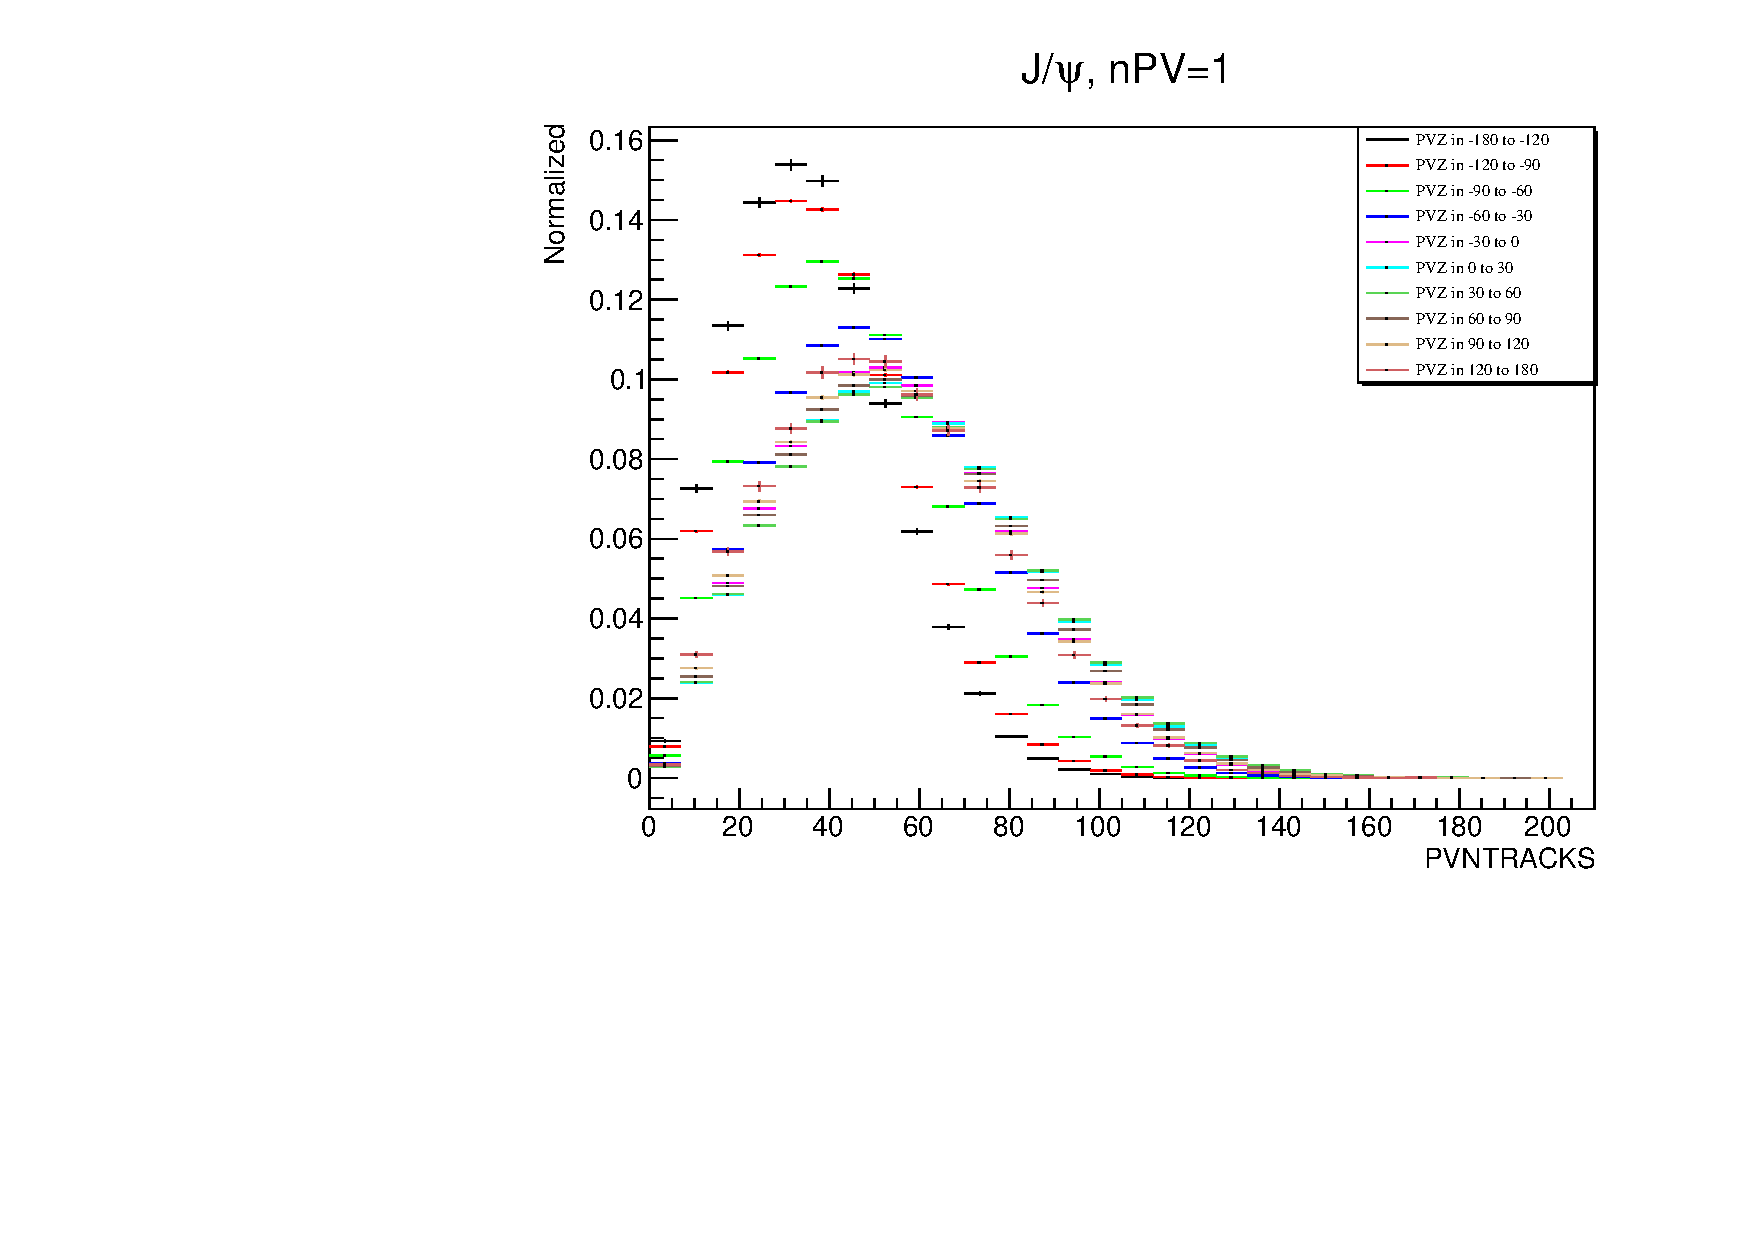
\includegraphics[width=0.49\linewidth]{Jpsi_PVZ_vs_PVNTRACKS}
      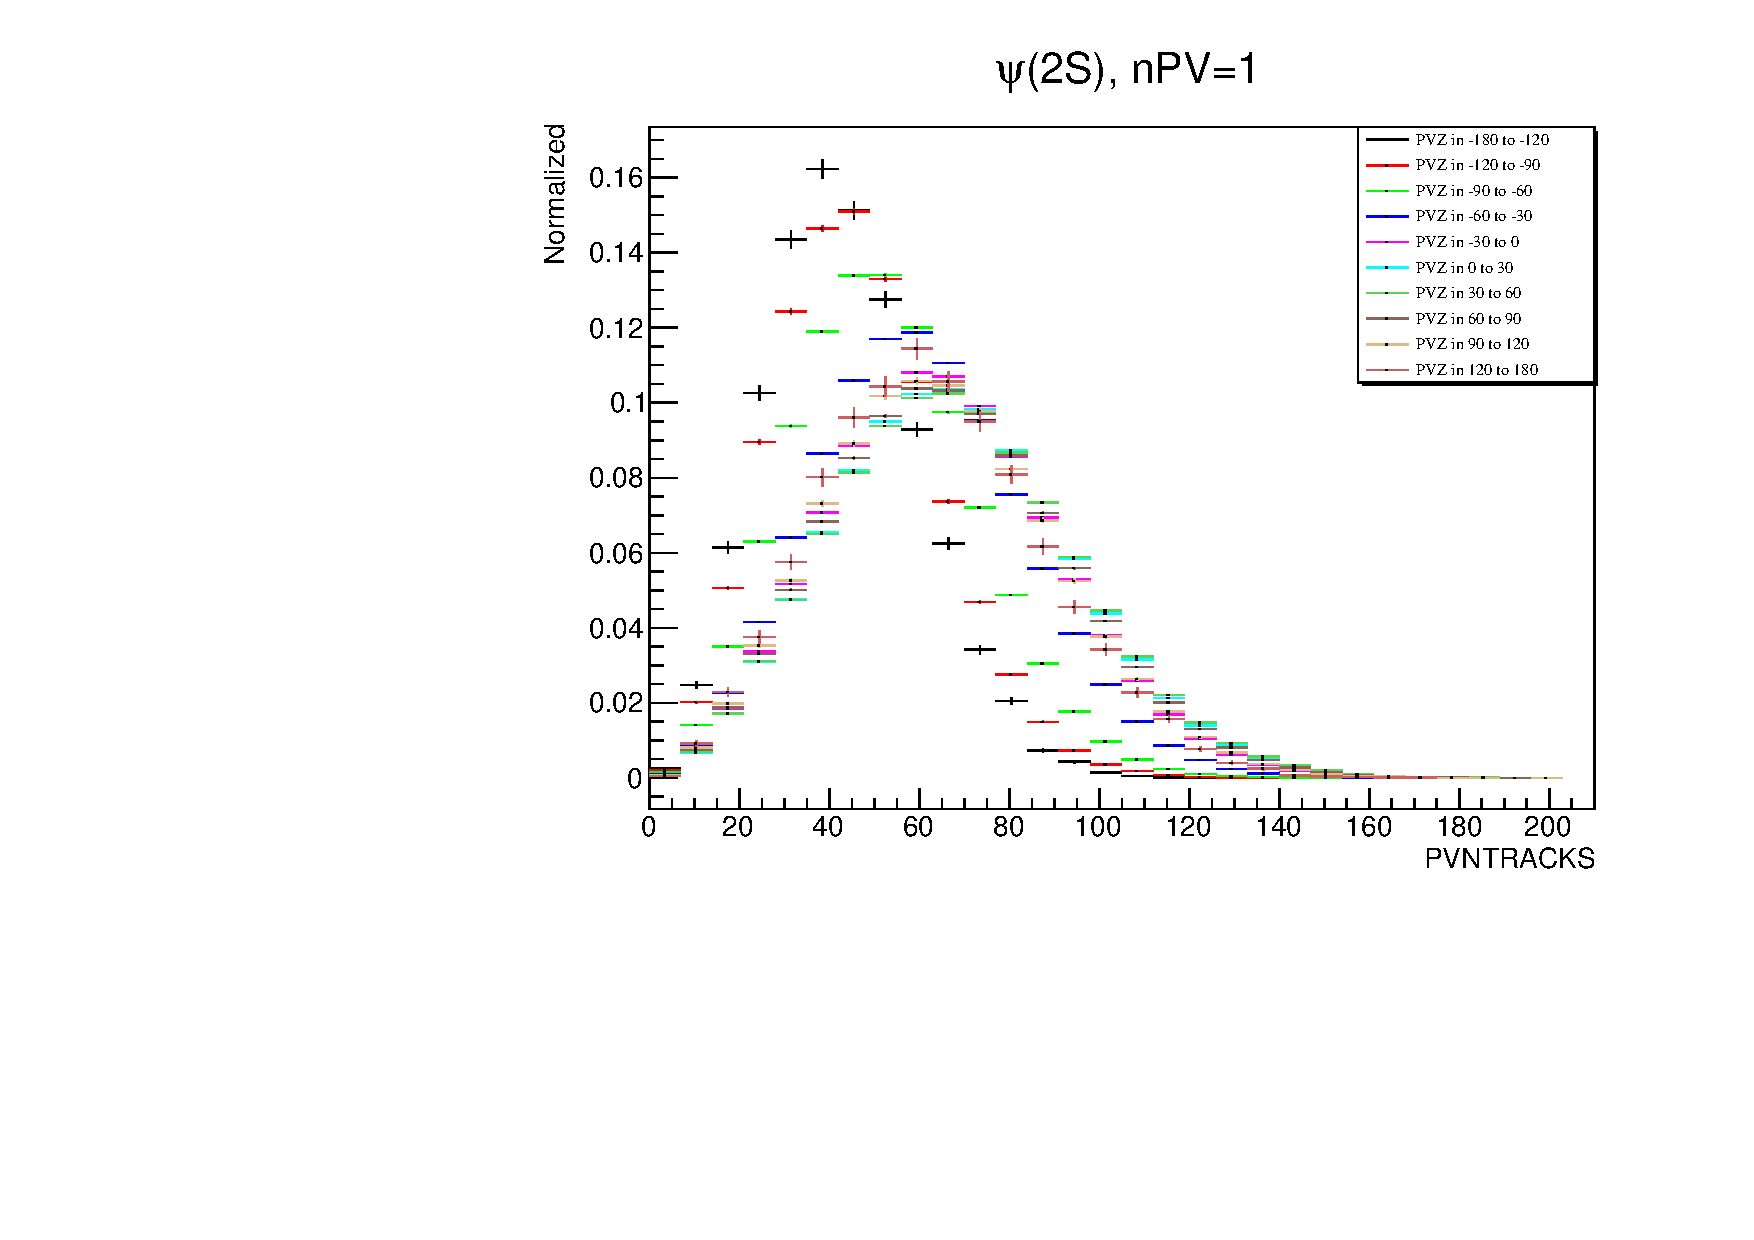
\includegraphics[width=0.49\linewidth]{Psi2S_PVZ_vs_PVNTRACKS}
      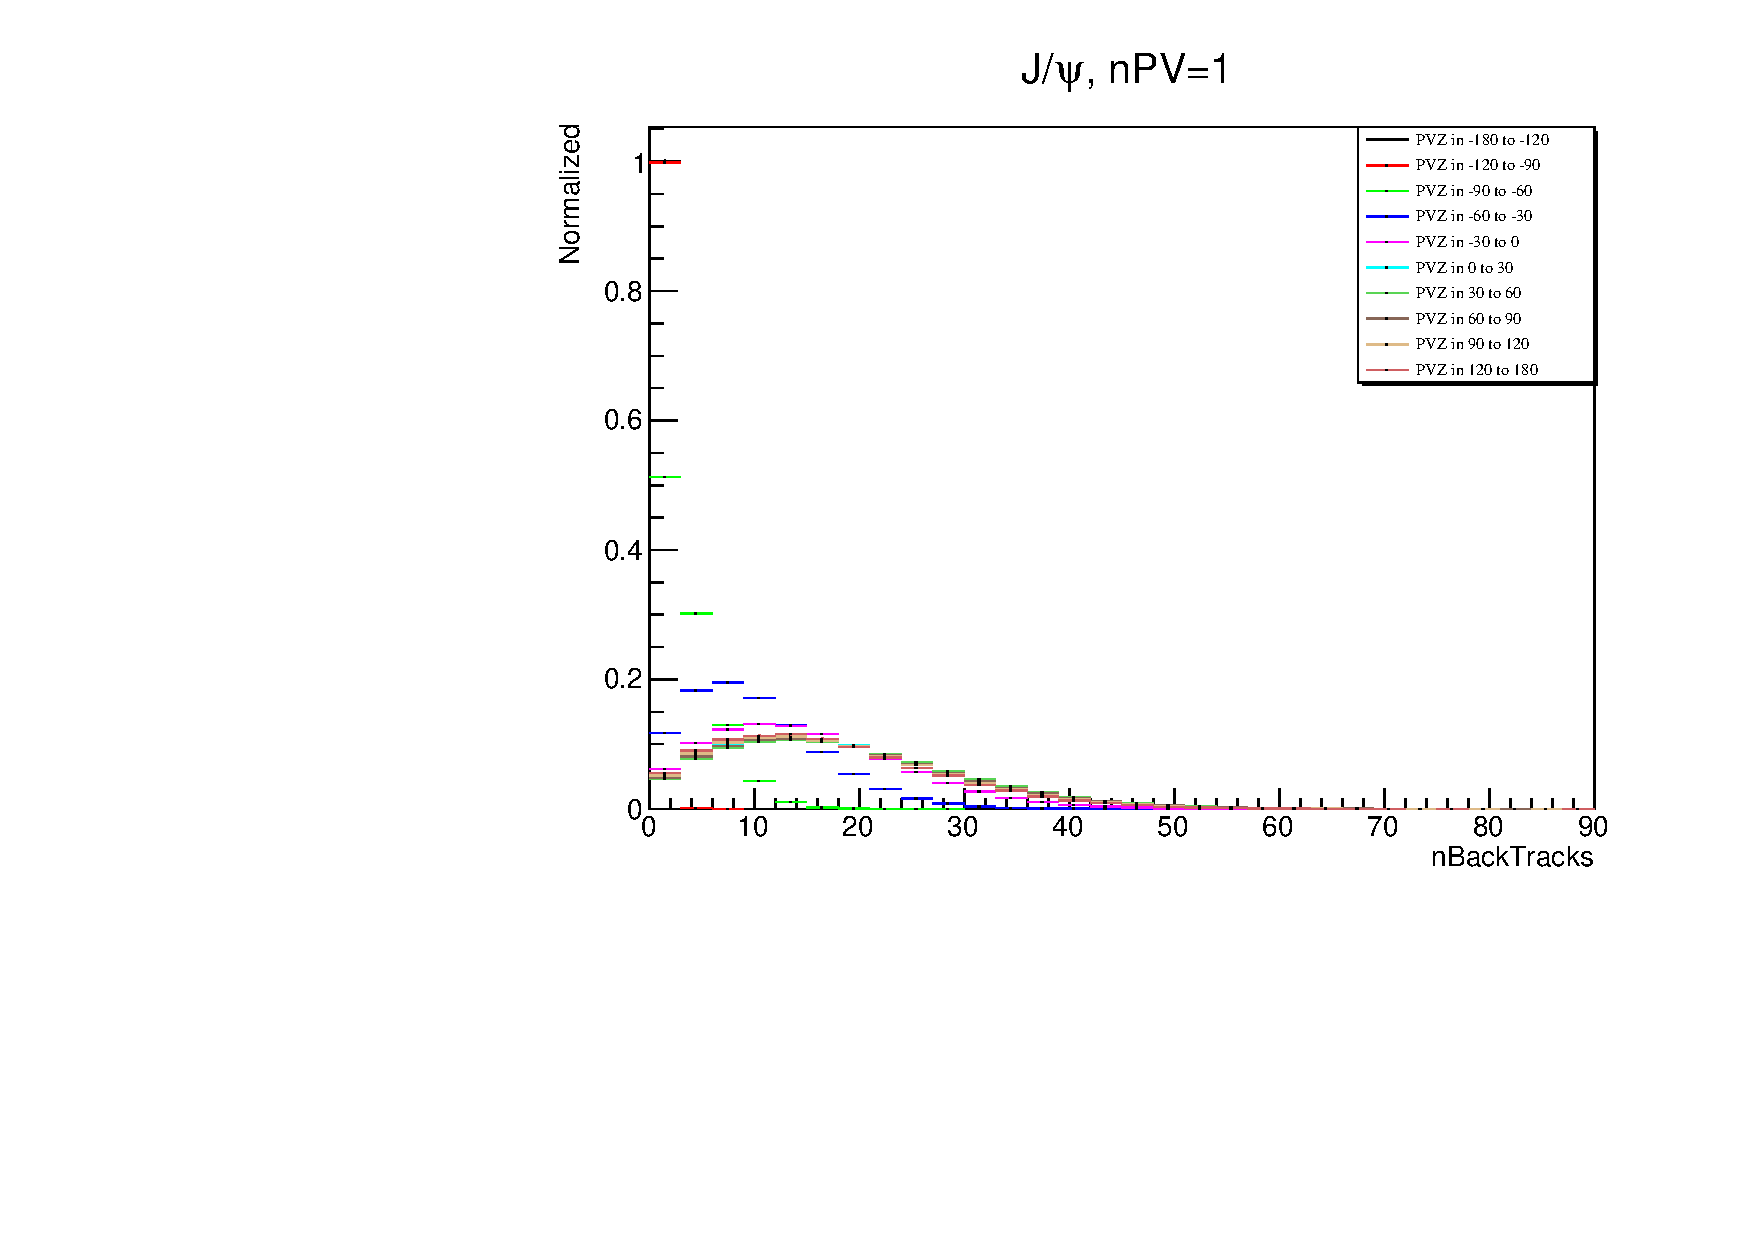
\includegraphics[width=0.49\linewidth]{Jpsi_PVZ_vs_nBackTracks}
      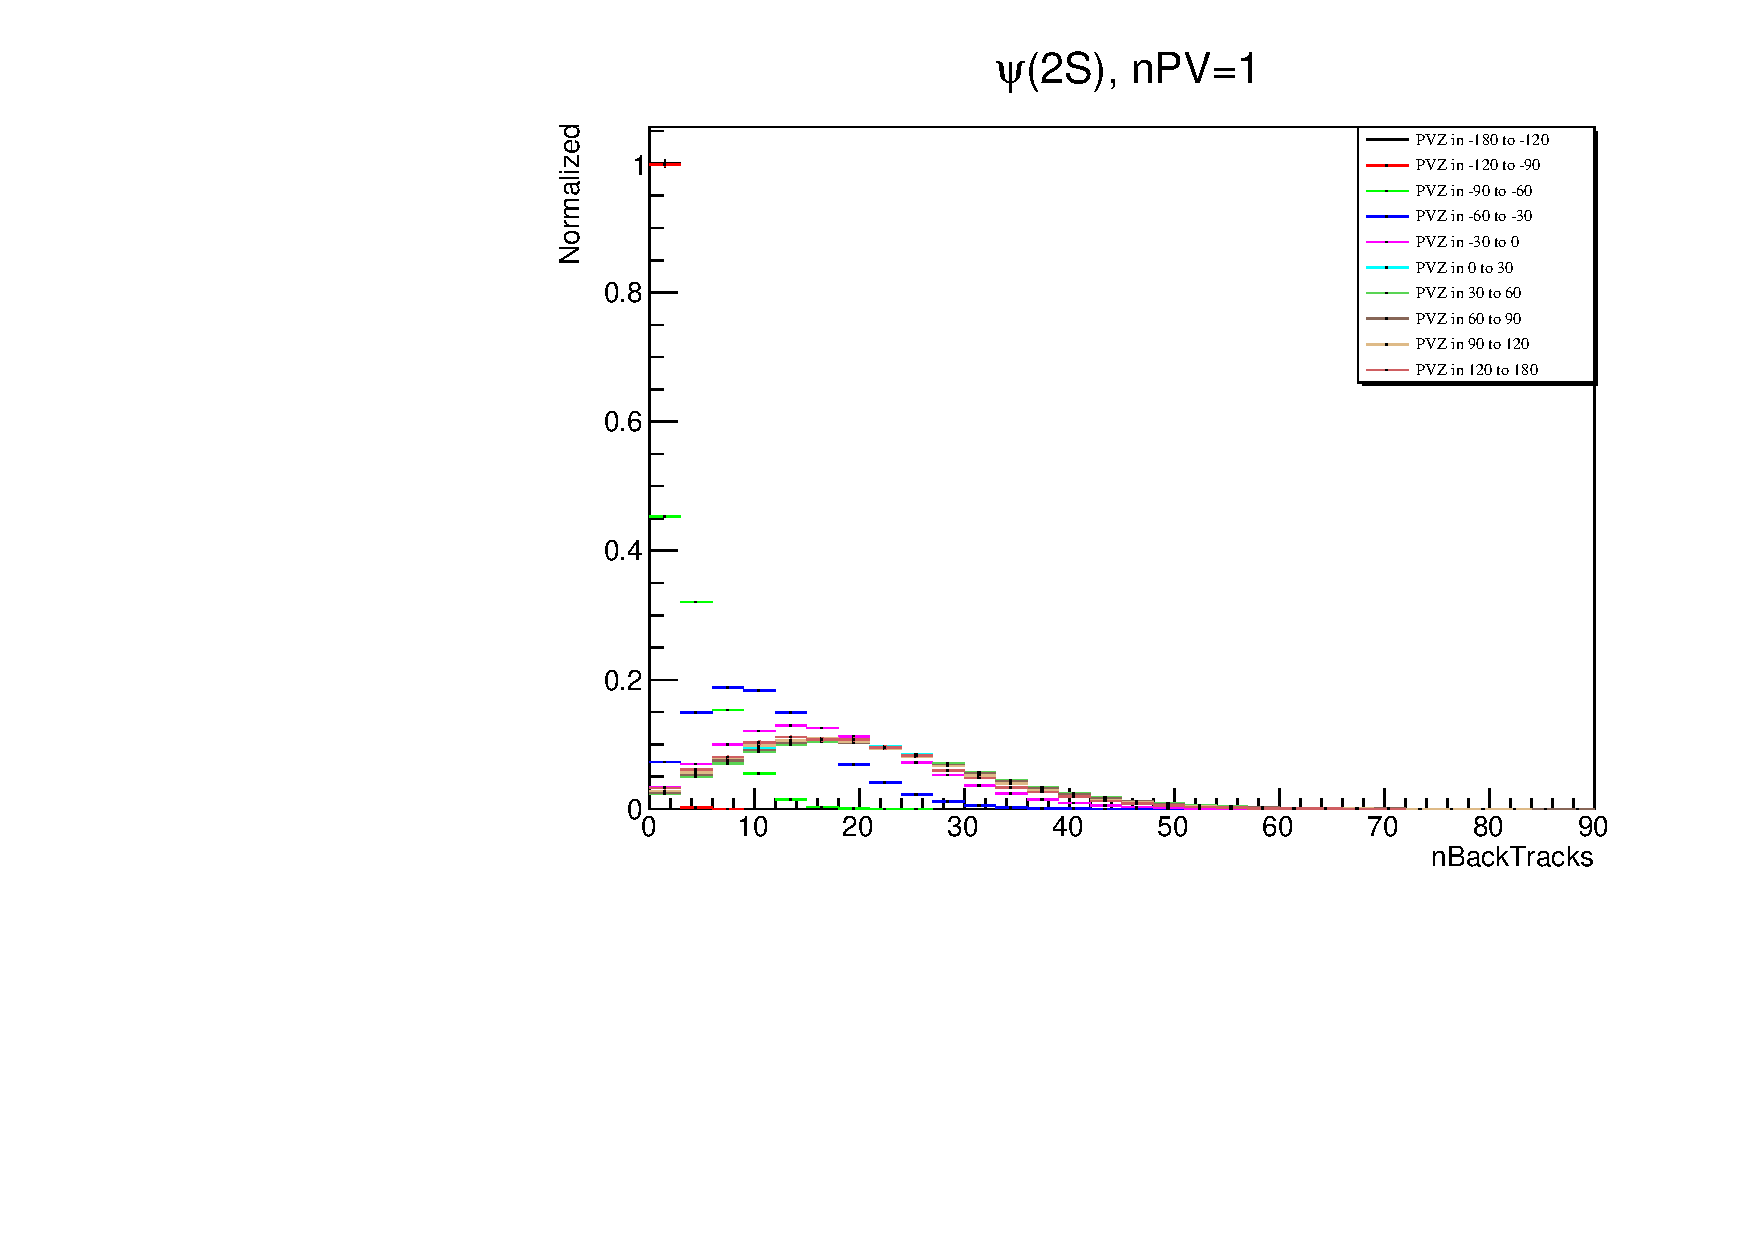
\includegraphics[width=0.49\linewidth]{Psi2S_PVZ_vs_nBackTracks}
      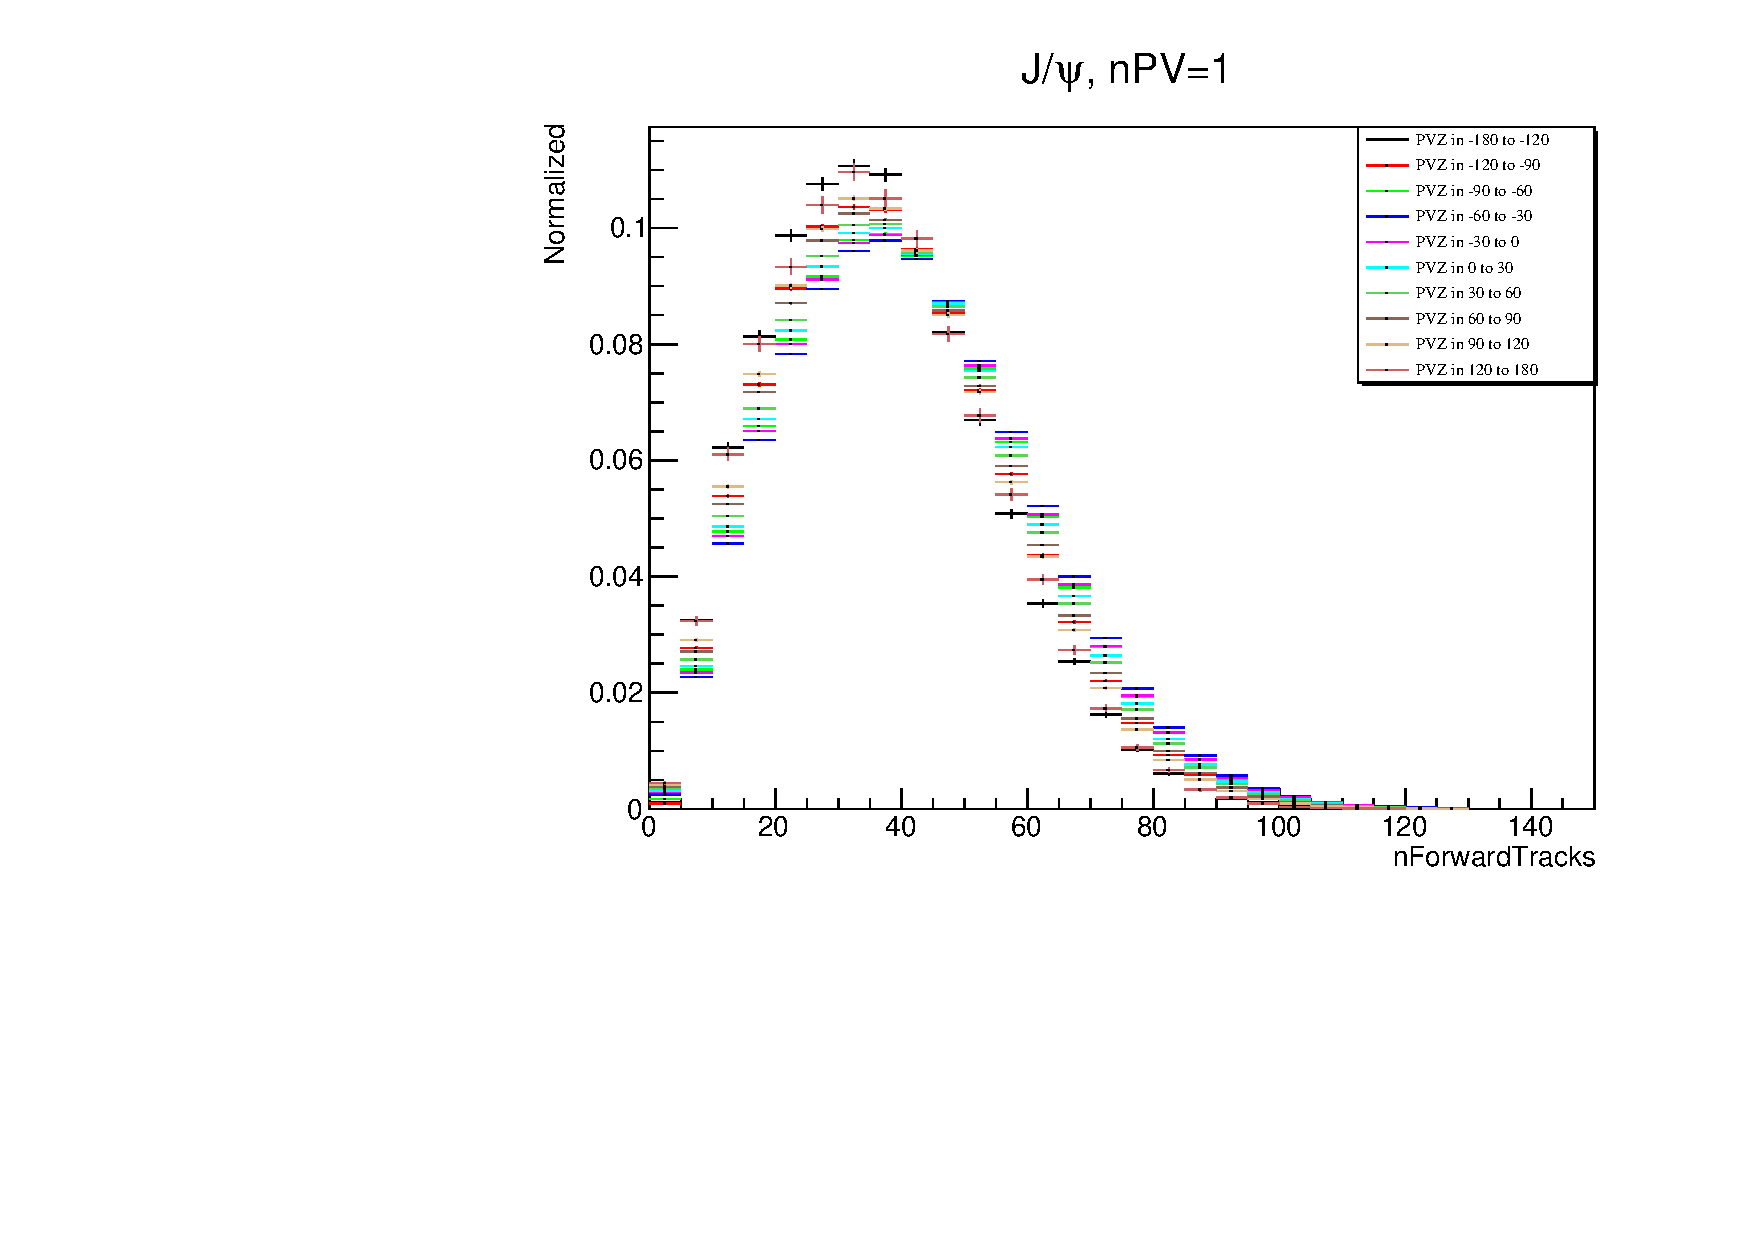
\includegraphics[width=0.49\linewidth]{Jpsi_PVZ_vs_nForwardTracks}
      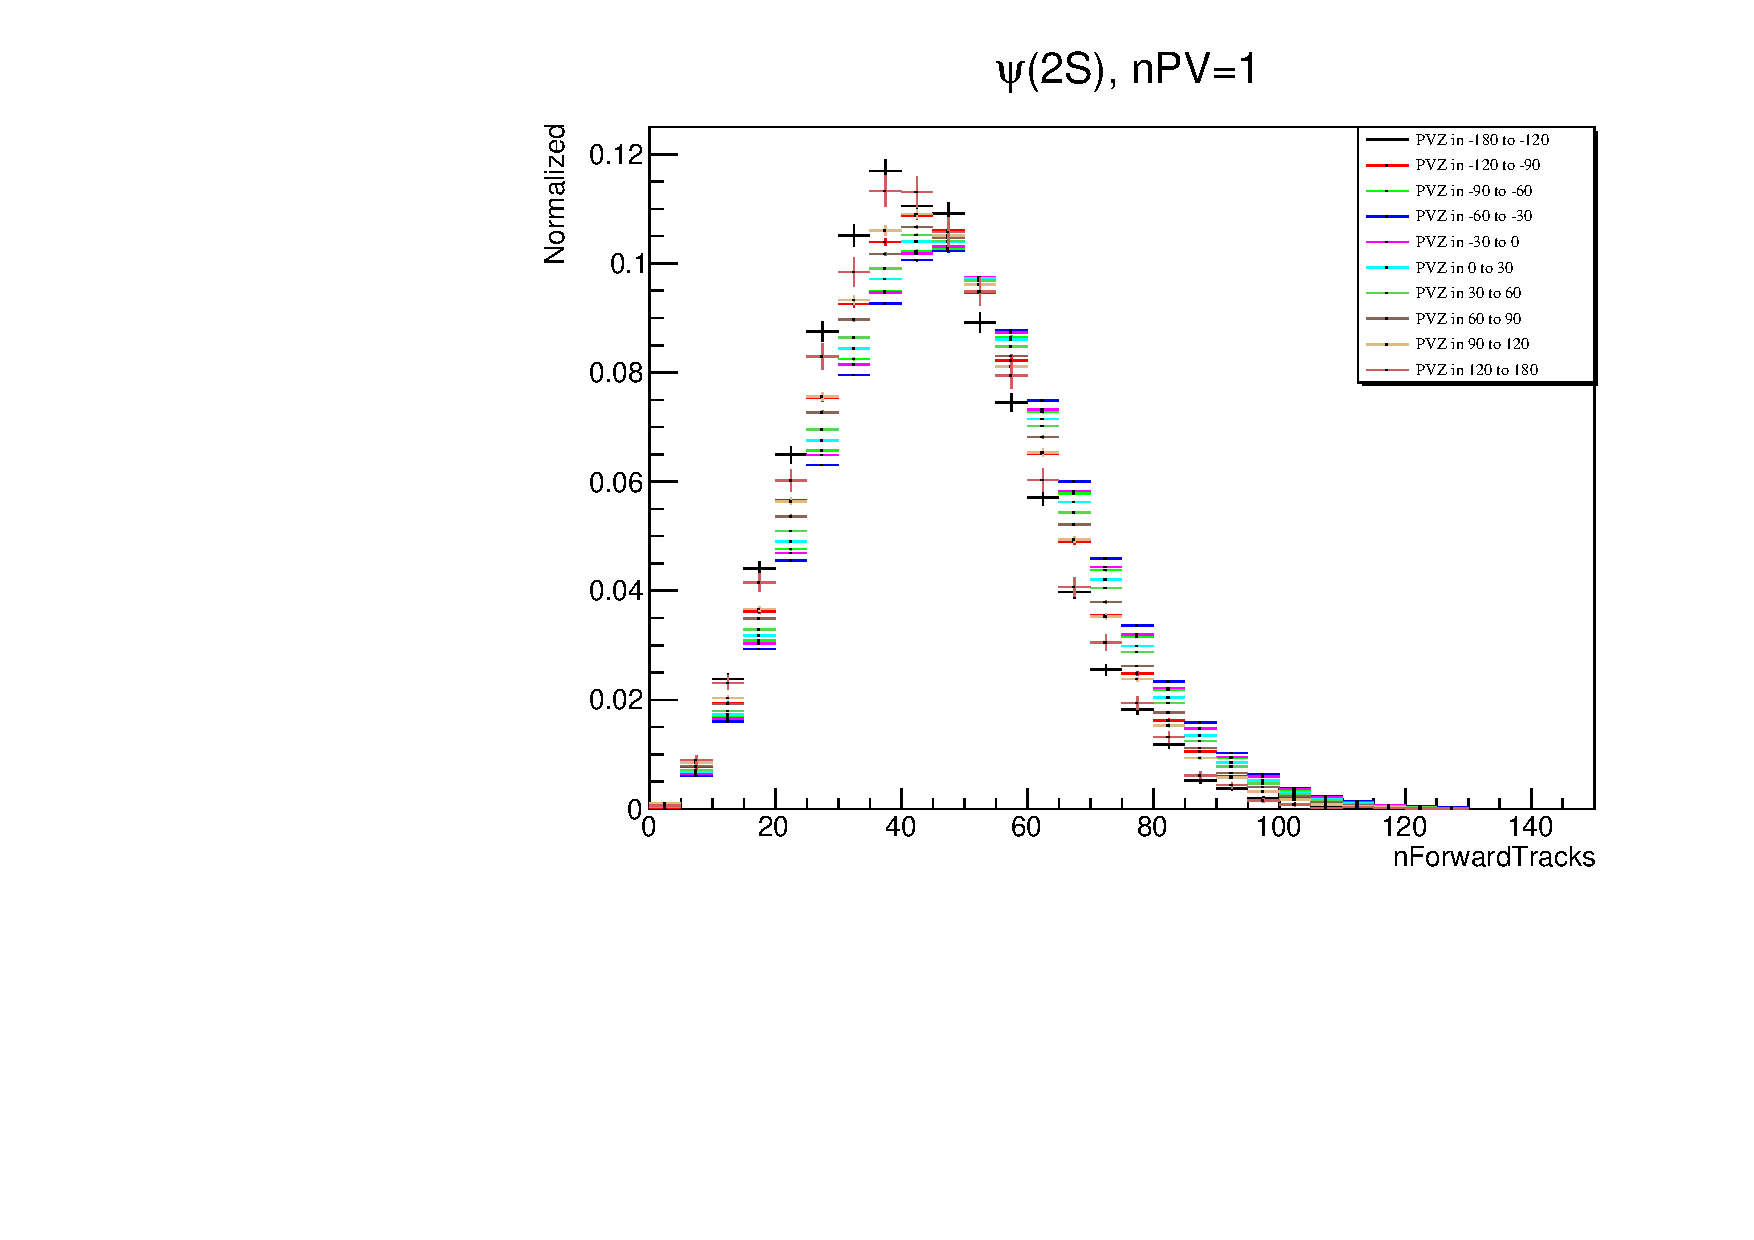
\includegraphics[width=0.49\linewidth]{Psi2S_PVZ_vs_nForwardTracks}
    \end{center}
    \caption{
    Distribution of PVNTRACKS, nBackTracks and nForwardTracks under nPVs $=1$ for $\jpsi$ (left) and $\psitwos$ (right). The clear deviation shows for $z_{\mathrm{PV}}$ smaller than a certain range so that we 
    subtract that part of data for equivalence of VELO acceptance.
      }
    \label{PVZvsPVNTRACKS}
  \end{figure}
